\documentclass{article}

\usepackage[utf8]{inputenc}
\usepackage{polski}
\usepackage{natbib}
\usepackage{graphicx}
\usepackage{tcolorbox}
\usepackage{geometry}
\usepackage{float}
\usepackage{listings}

\title{\textbf{AMBULANCE NAVIGATOR - specyfikacja implementacyjna}}
\author{Kamil Sztandur, Jakub Grenda, Robert Odrowąż-Sypniewski}
\date{14.12.2020}

\newcommand\tab[1][1cm]{\hspace*{#1}}
\lstset{frame=tb,
  aboveskip=3mm,
  belowskip=3mm,
  showstringspaces=false,
  columns=flexible,
  basicstyle={\small\ttfamily},
  numbers=none,
  numberstyle=\tiny\color{rgb}{0.5,0.5,0.5},
  keywordstyle=\color{rgb}{0.58,0,0.82}
  commentstyle=\color{rgb}{0,0.6,0},
  stringstyle=\color{mauve},
  breaklines=true,
  breakatwhitespace=true,
  tabsize=3
}

\begin{document}
\begin{tcolorbox}
\maketitle
\end{tcolorbox}
\newpage

\section{Informacje ogólne}
\subsection{Nazwa programu}
\tab Program nazywa się \textbf{Ambulance Navigator}.

\subsection{Poruszany problem}
\tab Problemem rozwiązywanym przez ten program jest zagadnienie rozlokowania chorych pacjentów w szpitalach w obrębie kraju w dobie pandemii. Ambulance Navigator skupia się na tym, aby każdemu pacjentowi zostało przyporządkowane wolne łóżko w możliwie najbliższym szpitalu lub skierowanie go na poczekalnię ostatniego odwiedzonego szpitala w przypadku przepełnienia wszystkich placówek.
\newline \tab Należy pamiętać, że głównym zadaniem programu jest symulacja podróży takich pacjentów według określonych protokołów, co pozwala zobaczyć i ocenić skuteczność ich działania. Program nie stanowi najlepszego rozwiązania problemu.

\subsection{Uruchomienie programu}
\tab Ambulance Navigator uruchamia się z poziomu graficznego eksploratora plików. Należy kliknąć lewym przyciskiem myszki na ikonę pliku:
\texttt{AmbulanceNavigator.exe} / \texttt{AmbulanceNavigator.app} / \texttt{AmbulanceNavigator}
(w zależności od systemu operacyjnego) w katalogu, w którym się on znajduje. Przewidywana jest kompatybilność z systemami operacyjnymi Windows, Linux oraz macOS.
\newline \tab Program jest aplikacją desktopową i uruchamia się w oknie. Hierarchia, wygląd i funkcjonalności poszczególnych okien zostały opisane w rozdziale poświęconemu interfejsowi graficznemu. Możliwa jest także implementacja webowa, ale nie jest ona wymagana w finalnym produkcie.

\subsection{Przyjmowanie danych przez program}
\tab Należy dokładnie przestudiować strukturę plików wejściowych na podstawie przedstawionych standardów na następnej stronie tego dokumentu, ponieważ wszelkie odstępstwa od ogólnoprzyjętych szablonów mogą spowodować nieprawidłową pracę, a nawet zatrzymanie pracy programu. Należy przestrzegać tych podstawowych zasada:
\begin{itemize}
    \item Liczby określające id powinny być \textbf{liczbami całkowitymi}.
    \item Współrzędne mogą być liczbami zmiennoprzecinkowymi, choć mogą pozostać całkowitymi.
    \item Nie należy pomijać bądź modyfikować \textbf{żadnych} nagłówków sekcji.
    \item Trzeba pamiętać o \textbf{jednowierszowych odstępach} pomiędzy każdymi sekcjami.
    \item Liczby zmiennoprzecinkowe należy zapisywać za pomocą \textbf{kropki} (np. 2.50).
\end{itemize}
\newpage

\subsection{Standardy plików wejściowych.}
\begin{tcolorbox}[title={Przykładowy plik zawierający dane szpitali, granic kraju i dróg miedzy szpitalami.}]
\# Szpitale (id $|$ nazwa $|$ wsp. x $|$ wsp. y $|$ Liczba łóżek $|$ Liczba wolnych łóżek)
\newline 1 $|$ Szpital Wojewódzki nr 997 $|$ 10 $|$ 10 $|$ 1000 $|$ 100
\newline 2 $|$ Krakowski Szpital Kliniczny $|$ 100 $|$ 120 $|$ 999 $|$ 99
\newline 3 $|$ Pierwszy Szpital im. Prezesa RP $|$ 120 $|$ 130 $|$ 99 $|$ 0
\newline 4 $|$ Drugi Szpital im. Naczelnika RP $|$ 10 $|$ 140 $|$ 70 $|$ 1
\newline 5 $|$ Trzeci Szpital im. Króla RP $|$ 140 $|$ 10 $|$ 996 $|$ 0
\newline 	
\newline \# Obiekty (id $|$ nazwa $|$ wsp. x $|$ wsp. y)
\newline 1 $|$ Pomnik Wikipedii $|$ -1 $|$ 50
\newline 2 $|$ Pomnik Fryderyka Chopina $|$ 110 $|$ 55
\newline 3 $|$ Pomnik Anonimowego Przechodnia $|$ 40 $|$ 70
\newline 
\newline \# Drogi (id $|$ id\textunderscore szpitala $|$ id\textunderscore szpitala $|$ odległość)
\newline 1 $|$ 1 $|$ 2 $|$ 700
\newline 2 $|$ 1 $|$ 4 $|$ 550
\newline 3 $|$ 1 $|$ 5 $|$ 800
\newline 4 $|$ 2 $|$ 3 $|$ 300
\newline 5 $|$ 2 $|$ 4 $|$ 550
\newline 6 $|$ 3 $|$ 5 $|$ 600
\newline 7 $|$ 4 $|$ 5 $|$ 750
\end{tcolorbox}

\begin{tcolorbox}[title={Przykładowy plik zawierający dane pacjentów potrzebujących wolnego łóżka w szpitalu.}]
\# Pacjenci (id $|$ wsp. x $|$ wsp.y)
\newline 1 $|$ 20 $|$ 20
\newline 2 $|$ 99 $|$ 105
\newline 3 $|$ 23 $|$ 40
\end{tcolorbox}
\newpage

\section{Opis pakietów i modułów}
\subsection{Struktura pakietów i modułów.}
\begin{figure}[H]
    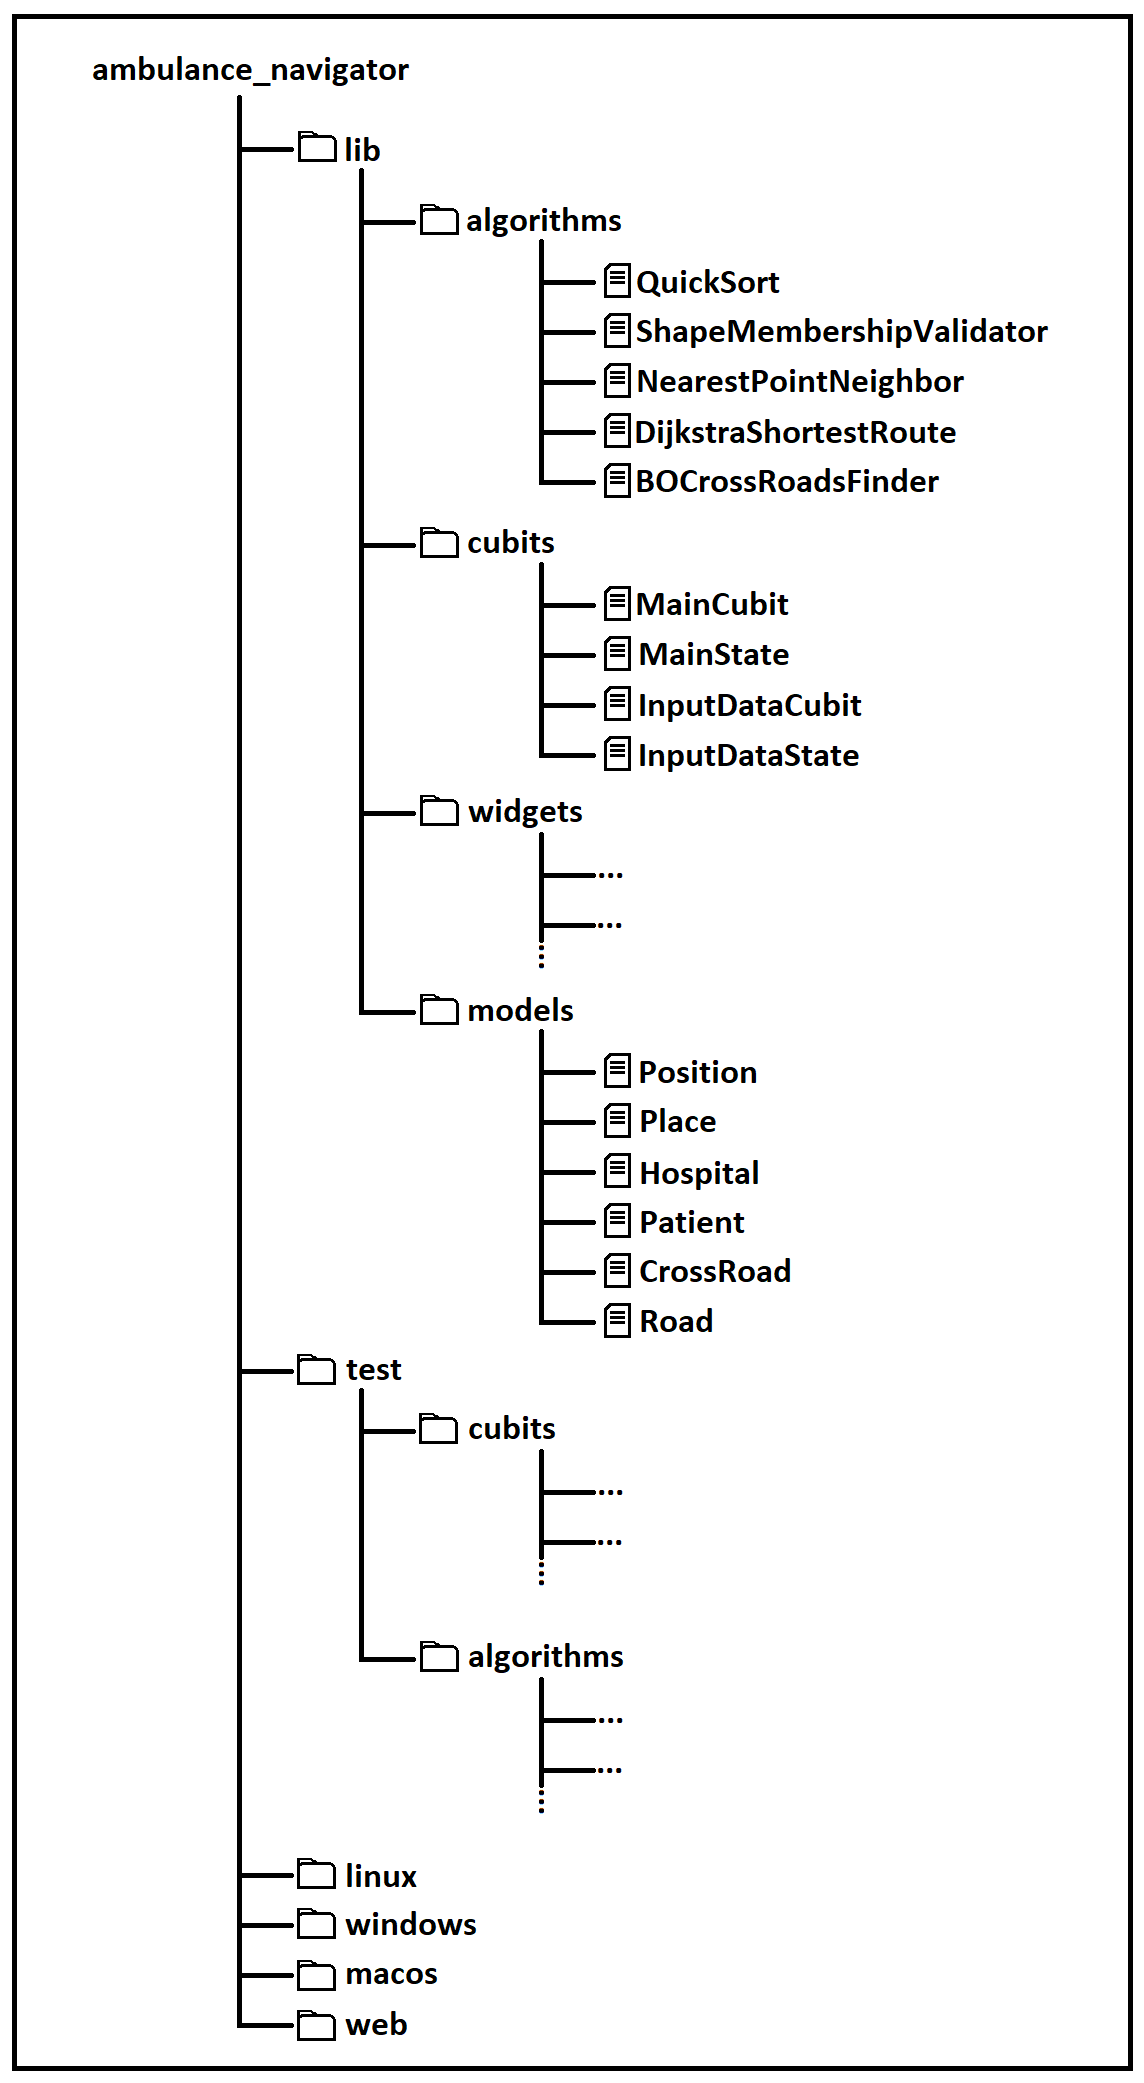
\includegraphics[width=10cm]{packages.png}
    \centering
\end{figure}
\newpage

\subsection{Pakiet główny \texttt{ambulance\_navigator}}
Ten pakiet jest głównym pakietem programu. Zawiera wszystko to, z czego składa się program:
\begin{itemize}
\item \textbf{lib} - pakiet właściwy stanowiący ten program. Zawiera wszystkie opisane w dalszej części pakiety i klasy programu.
\item \textbf{test} - Pakiet zawierający testy jednostkowe poszczególnych modułów aplikacji.
\item \textbf{linux} - pakiet odpowiedzialny za wrapper applikacji dla systemu Linux.
\item \textbf{windows} - pakiet odpowiedzialny za wrapper applikacji dla systemu Windows.
\item \textbf{macos} - pakiet odpowiedzialny za wrapper applikacji dla systemu macOS.
\item \textbf{web} - pakiet zawierający statyczne pliki aplikacji webowej.
\end{itemize}

\subsubsection{Pakiet \texttt{ambulance\_navigator/lib}}
Ten pakiet jest pakietem właściwym stanowiącym logikę programu. Zawiera wszystkie pakiety i klasy stanowiące logikę bizensową i interfejs graficzny aplikacji.
\begin{itemize}
\item \textbf{algorithms} - podpakiet zawierający wszystkie algorytmy wykorzystane w programie.
\item \textbf{widgets} - podpakiet zawierający widget wykorzystywane w aplikacji.
\item \textbf{cubits} - podpakiet zawierający klasy logiki stanu aplikacji.
\item \textbf{models} - podpakiet zawierający obiekty modeli używanych w programie przedstawiających interesujące nas realne obiekty, o których traktuje program.
\end{itemize}

\subsubsection{Pakiet \texttt{ambulance\_navigator/lib/algorithms}}
Pakiet zawierający wszystkie algorytmy wykorzystane w programie.
\begin{itemize}
\item \textbf{QuickSort} - moduł zawierający algorytm iteracyjnego sortowania szybkiego, wybierający oś podziału poprzez medianę.

\item \textbf{ShapeMembershipValidator} - moduł zawierający algorytm rozpoznający, czy podany punkt zawiera się we wnętrzu figury o podanym kształcie. Kształt figury określa tablica obiektów  Point. Jest wykorzystywany do sprawdzenia, czy oczekujący pacjent znajduje się poza granicami kraju.

\item \textbf{NearestPointNeighbor} - moduł zawierający algorytm odnajdujący najbliższego sąsiada podanego punktu. Jest wykorzystywany do odnalezienia najbliższego szpitala po odebraniu pacjenta przez karetkę pogotowia lub po dotarciu do szpitala, w którym brakuje wolnych łóżek.

\item \textbf{DijkstraShortestRoute} - moduł zawierający algorytm Dijkstry odnajdujący połączenie pomiędzy dwoma punktami o najmniejszej wadze. Jest wykorzystywany do sprawdzenia, którą drogą należy się udać, aby jak najszybciej dotrzeć do innego szpitala.

\item \textbf{BOCrossRoadsFinder} - moduł zawierający algorytm Benttleya-Ottmana odnajdujący skrzyżowania dróg pomiędzy szpitalami, co utworzy nowe potencjalne trasy dla karetek pogotowia. W przypadku porażki implementacji tego algorytmu w finalnym produkcie może go zastąpić algorytm własny, brutalnie odnajdujący takie skrzyżowania.
\end{itemize}

\subsubsection{Pakiet \texttt{ambulance\_navigator/lib/cubits}}
Pakiet zawierający zbiór klas stanowiących logikę stanu aplikacji.
\begin{itemize}
\item \textbf{MainCubit} - Główna klasa zarządzająca stanem aplikacji. Rozszerza \texttt{Cubit<MainState>}.
\item \textbf{MainState} - Abstrakcyjna klasa której rozszerzenia stanowią możliwe stany aplikacji.
\item \textbf{InputDataCubit} - Klasa odpowiedzlana za wczytywanie i przechowywanie dancyh wejściowych. Rozszerza \texttt{Cubit<InputDataState>}.
\item \textbf{InputDataState} - Abstrakcyjna klasa której rozszerzenia stanowią możliwe stany danych wejściowych.
\end{itemize}

\subsubsection{Pakiet \texttt{ambulance\_navigator/lib/widgets}}
Pakiet zawierający widgety stanowiące elementy interfejsu graficznego aplikacji. Klasy zawerte w typ pakiecie wypiasne są w sekcji "Struktura interfejsu graficznego".

\subsubsection{Pakiet \texttt{ambulance\_navigator/lib/models}}
Pakiet zawierający obiekty modeli używanych w programie przedstawiających interesujące nas obiekty o których traktuje program.
\begin{itemize}
\item \textbf{Position} - klasa reprezentująca punkt na płaszczyźnie kartezjańskiej.

\item \textbf{Place} - klasa reprezentująca obiekt punktu granicznego (określa granice kraju), zawiera id, nazwę i koordynaty. Dziedziczy po klasie Position.

\item \textbf{Hospital} - klasa reprezentujący obiekt szpitala, dziedziczy po klasie Place. Może określać granice kraju. Zawiera swoje id, nazwę, koordynaty, liczbę wszystkich/wolnych łóżek oraz liczbę pacjentów, czekających na przyjęcie przed wejściem.

\item \textbf{Patient} - klasa reprezentujący obiekt pacjenta, który potrzebuje wolnego łóżka w szpitalu. Zawiera swoje id oraz koordynaty. Opcjonalnie powinien zawierać listę numerów id szpitali, które odwiedził (a nie dostał łóżka). Dziedziczy po klasie Position.

\item \textbf{CrossRoad} - moduł reprezentujący skrzyżowanie dróg międzyszpitalnych, na którym może skręcić karetka pogotowia. Dziedziczy po klasie Position.

\item \textbf{Road} - moduł reprezentujący drogę, po której może poruszać się karetka z pacjentem w czasie transportu między szpitalami (ta zasada nie obowiązuje w czasie dostarczania pacjenta do pierwszego szpitala).
\end{itemize}

\subsubsection{Pakiet \texttt{ambulance\_navigator/test}}
Pakiet zawierający testy jednostkowe poszczególnych modułów aplikacji.
\begin{itemize}
\item \textbf{cubits} - pakiet zawierający testy jednostkowe klas stanowiących logikę stanu aplikacji.
\item \textbf{algorithms} - pakiet zawierający testy jednoskowe algorytmów wykorzystywanych w aplikacji.
\end{itemize}
Przyjęte konwencje i sposób pisania testów jednostkowych został opisany w rozdziale poświęconym testowaniu.

\section{Opis klas algorytmów i struktur danych}
\subsection{Algorytm Sortowania Szybkiego}
\tab Algorytm sortowania zawarty w klasie QuickSort jest oparty na iteracyjnym algorytmie szybkiego sortowania QuickSort wzbogaconego o wybieranie osi podziału (pivota) poprzez medianę trzech wartości, czyli wartości o pierwszym i ostatnim indeksie w wektorze oraz losowej z pomiędzy nich. Takie rozwiązanie znacznie amortyzuje złożoność algorytmu przy pesymistycznych danych i zmniejsza prawdopodobieństwo na wystąpienie przypadku pesymistycznego, kiedy za oś podziału wybierana jest skrajna wartość co wydłuża proces sortowania. Dzieje się tak, ponieważ QuickSort najlepiej spisuje się, gdy w wyniku podziału wektora powstają dwa jak najbardziej równe podwektory. Zmniejsza to liczbę potrzebnych iteracji. W przypadku ciągłego wybierania skrajnych wartości czas potrzebny na posortowanie listy wzrasta drastycznie. 
\newline \tab Złożoność obliczeniowa typowego przypadku jest równa: $O_{(N)} = n \cdot log(n)$, a przypadku pesymistycznym (którego szansa na wystąpienie została znacznie zredukowana) $O_{(N)} = n^2$. 
\newline \tab Do rozwiązania problemu sortowania został użyty QuickSort, ponieważ do pracy na takich danych jakie będzie musiał w tym programie pracować powinien sprawdzać się dobrze. Istnieje praktycznie zerowa szansa, że wszystkie odległości przyjmą tę samą wartość bądź, że będą już posortowane w danych wejściowych. Jest sytuacja tak małoprawdopodobna i niesamowicie wyjątkowa, że nie warto jej nawet rozważać. W przypadku jej wystąpienia złożoność obliczeniowa została zredukowana dzięki opisanemu wyborowi osi podzialu poprzez medianę.

\subsection{Algorytm przynależności punktu do figury}
\tab Algorytm ma na celu określenie, czy dany punkt leży wewnątrz danej figury na płaszczyźnie kartezjańskiej. Kształt badanej figury określa tablica zawierająca punkty, które definiują jej rozpiętość. Algorytm zwraca wartość prawda/fałsz, oznaczającą wynik testu na przynależność podanego punktu do wskazanej figury.
\newline \tab Działanie algorytmu polega na podziale otrzymanej figury na trójkątne poligony tak, aby pokryły one całe pole figury przy równoczesnym zachowaniu ich optymalnej liczby. Następnie dla każdego poligonu wykonywany jest test na przynależność podanego punktu do niego. W przypadku wykrycia przynależności punktu do jednego z poligonów figury algorytm przerywa działanie i zwraca wartość \textit{prawda}. W przypadku sprawdzenia wszystkich poligonów i nieodnalezienia przynależności punktu do żadnego z nich algorytm zwraca wartość \textit{fałsz}.
\newline \tab Test na przynależność podanego punktu do trójkątnego poligonu oparte jest na horyzontalnym przesuwaniu kursora począwszy od koordynatów badanego punktu oraz zliczanie, ile razy kursor przeciął granicę poligonu (na podstawie funkcji matematycznych). Jeżeli liczba przeciętych granic jest nieparzysta lub punkt leży na jednej z takich krawędzi, to oznacza że punkt leży wewnątrz poligonu. Jeżeli liczba przeciętych granic jest parzysta, to znaczy że punkt leży poza poligonem.
\begin{figure}[H]
    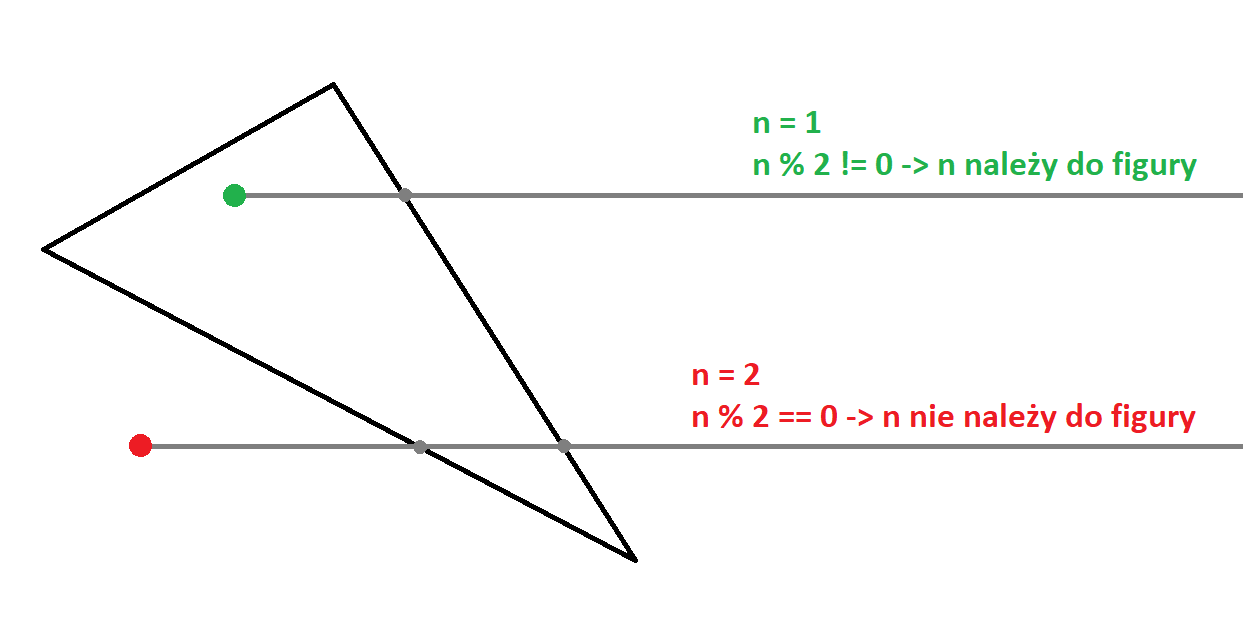
\includegraphics[width=12cm]{MembershipTest.png}
    \centering
\end{figure}
\tab W momencie pisania tej specyfikacji algorytm podziału figury na poligony jest oparty na brute force i posiada nieoptymalną złożoność obliczeniową $O(n^3)$, gdzie n to liczba punktów określających kształt figury. Cały problem złożoności polega na idealnym dobraniu sposobu podzialu figury na poligony tak, aby pokryć ją całą, ale równocześnie zachować rozsądną liczbę poligonów. Cierpi też na sporadyczne błędy wynikające z zaokrągleń liczb zmiennoprzecinkowych, co będzie musiało zostać usprawnione w procesie implementacji.
\begin{figure}[H]
    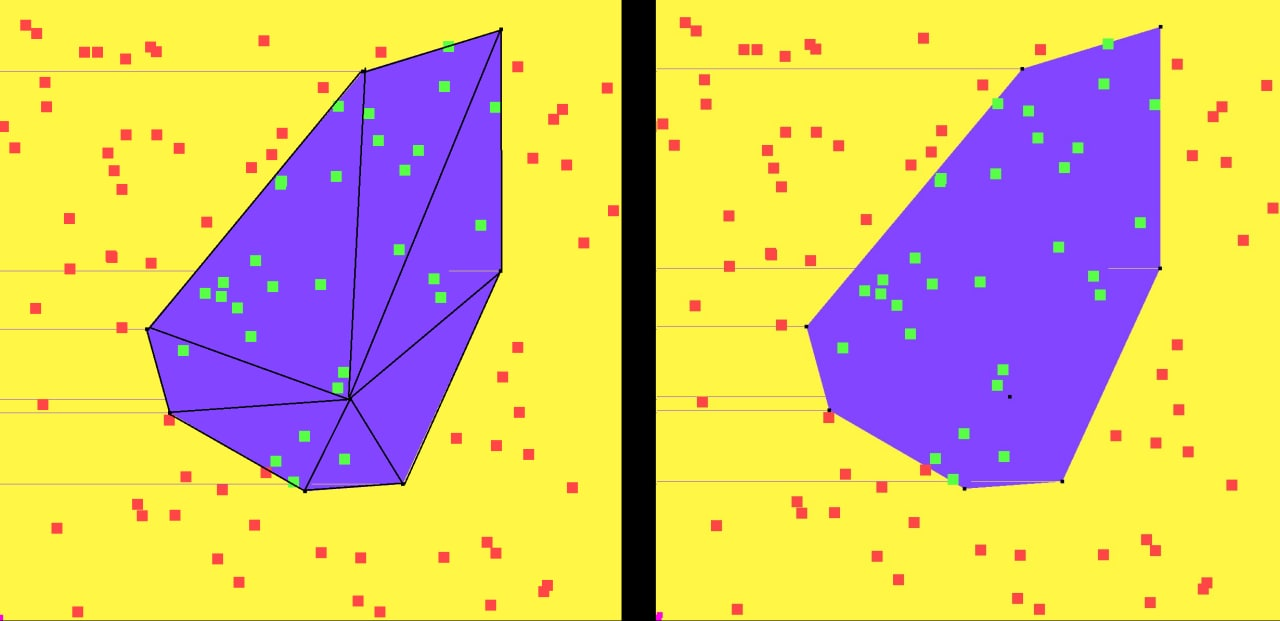
\includegraphics[width=15cm]{Subpolygons.png}
    \centering
    \caption {Wynik symulacji pracy algorytmu w środowisku Java. Po lewej optymalny podział na poligony. Po prawej figura bez podziału. Artefakty na obrazie w postaci horyzontalnych linii nie są winą pracy algorytmu.}
\end{figure}
\tab Algorytm wykorzystywany jest do określania, czy pacjent znajduje się w granicach kraju, które są określane przez punkty graniczne.

\subsection{Uproszczony Algorytm Najbliższego Sąsiada}
\tab Uproszczona wersja (na potrzeby tak prostego problemu) algorytmu najbliższego sąsiada rozwiązującego problem tzw. komiwojażera, czyli określenia drogi przez wszystkie wierzchołki grafu tak, aby każdy następny odwiedzony wierzchołek był najbliższy aktualnemu, w którym znajduje się komiwojażer, ale równocześnie nie mógł on odwiedzić żadnego wierzchołka więcej niż jeden raz.
\newline \tab Komiwojażerem będzie karetka pogotowia wioząca pacjenta z jego domu do pierwszego najbliższego szpitala w linii prostej. Uproszczona wersja tego algorytmu nie będzie operować na grafie, lecz na płaszczyźnie kartezjańskiej stanowiącej mapę kraju. Zadaniem algorytmu będzie określenie, który szpital znajduje się najbliżej miejsca odebrania chorego pacjenta z domu przez karetkę.
\newline \tab Algorytm będzie liczyć bezwzględne odległości pomiędzy miejscem odebrania pacjenta, a koordynatami wszystkich n szpitali, co definiuje jego złożoność złożoność $O(n)$, gdzie $n$ to liczba szpitali w obrębie kraju.

\subsection{Algorytm Dijkstry}
\tab Podobnie jak algorytm najbliższego sąsiada służy do odnajdywania najkrótszej ścieżki w grafie. Często wykorzystuje się go w mapach satelitarnych do wyznaczania najkrótszej drogi do danych miejscowości, co świadczy o jego skuteczności w zadaniu przedstawionym przez ten program.
\tab Podróżnikiem po grafie będzie karetka pogotowia wioząca pacjenta do kolejnych szpitali w poszukiwaniu wolnego łóżka. Złożoność takiego algorytmu z wykorzystaniem naiwnej implementacji jest równa $O(n^2)$, gdzie n to liczba szpitali, między którymi pacjent może podróżować.
\newline \tab Ostatecznie w programie zostanie użyty albo ten algorytm, albo algorytm najbliższego sąsiada.

\subsection{Algorytm odnajdywania skrzyżowań Benttleya-Ottomanna (lub własny)}
\tab Algorytm Benttleya-Ottmana służy do odnajdywania skrzyżowań w danym zbiorze linii prostych. Znajduje taki punkt przecięcia się segmentów dwóch linii, aby nie był on punktem stykania się ich końców. Jego złożoność czasowa wynosi zaledwie $O((n + \frac{n^2}{log_n}) \cdot log_n$), gdzie n to liczba wszystkich linii. 
\newline \tab W przypadku porażki implementacji tego algorytmu w finalnym produkcie może go zastąpić algorytm własny, brutalnie odnajdujący takie skrzyżowania o złożoności $O(n^2)$, gdzie n to liczba wszystkich linii.

\newpage
\section{Logika interfejsu graficznego}
Logika i zarządzanie stanem w aplikacji zbudwane są zgodnie z architekturą BLoC przy użyciu bibiliotek \texttt{bloc} oraz \texttt{flutter\_bloc}. Logika zarządzająca stanem aplikacji podzielona jest na 2 cubity. Pierwszy z nich - \texttt{InputDataCubit} odpowiedzialny jest za obsługę wczytywania i przechowywanie danych wejsciowych. Drugi nadrzeędny cubit - \texttt{MainCubit} odpowiedzialny jest za sterowanie wykonywaniem symulacji. Ponieważ logika wydzielona jest do cubitów callbacki sprowadzają się do wywołania odpowienich method na jednym z 2 cubitów.

\section{Struktura interfejsu graficznego}
Ponieważ intefrejs programu oparty jest o framework Flutter jego struktura stanowi drzewo widgetów. Widgety nie nie będzące wejściami lub wyjściami programu, odpowiedzilane jedynie za layout i styl zostały pominięte z diagramu dla zachowania czytelności. \newline

\texttt{MainPage} \newline
\tab\texttt{InputDataMenu} \newline
\tab\tab\texttt{RaisedButton} (wybór pliku obiektów) \newline
\tab\tab\texttt{HospitalsList} \newline
\tab\tab\tab\texttt{Text} (tytuł listy) \newline
\tab\tab\tab\texttt{ListView} \newline
\tab\tab\tab\tab\texttt{ObjectListItem} \newline
\tab\tab\tab\tab\tab\texttt{Text} (indeks) \newline
\tab\tab\tab\tab\tab\texttt{Text} (nazwa) \newline
\tab\tab\tab\tab\tab\texttt{Text} (pozycja) \newline
\tab\tab\tab\tab\tab\texttt{IconButton} (widoczność) \newline
\tab\tab\texttt{ObjectsList} \newline
\tab\tab\tab\texttt{Text} (tytuł listy) \newline
\tab\tab\tab\texttt{ListView} \newline
\tab\tab\tab\tab\texttt{ObjectListItem} \newline
\tab\tab\tab\tab\tab\texttt{Text} (indeks) \newline
\tab\tab\tab\tab\tab\texttt{Text} (nazwa) \newline
\tab\tab\tab\tab\tab\texttt{Text} (pozycja) \newline
\tab\tab\tab\tab\tab\texttt{IconButton} (widoczność) \newline
\tab\tab\texttt{RaisedButton} (wybór pliku pacjentów) \newline
\tab\tab\texttt{PatientsList} \newline
\tab\tab\tab\texttt{Text} (tytuł listy) \newline
\tab\tab\tab\texttt{ListView} \newline
\tab\tab\tab\tab\texttt{PatientListItem} \newline
\tab\tab\tab\tab\tab\texttt{Text} (indeks) \newline
\tab\tab\tab\tab\tab\texttt{Text} (pozycja) \newline
\tab\tab\texttt{PatientInput} \newline
\tab\tab\tab\texttt{TextFormField} (pozycja x) \newline
\tab\tab\tab\texttt{TextFormField} (pozycja y) \newline
\tab\tab\tab\texttt{IconButton} (dodanie pacjenta) \newline
\tab\texttt{Stack} \newline
\tab\tab\texttt{MapView} \newline
\tab\tab\texttt{SimulationControls} \newline
\tab\tab\tab\texttt{FloatingActionButton} (uruchamianie i zatrzymywanie symulacji) \newline
\tab\tab\tab\texttt{FloatingActionButton} (resetowanie symulacji) \newline
\tab\tab\tab\texttt{Slider} (regulacja prędkości symulacji) \newline
\tab\texttt{LogList} \newline
\tab\tab\texttt{Text} (tytuł listy) \newline
\tab\tab\texttt{ListView} \newline
\tab\tab\tab\texttt{LogListItem} \newline
\tab\tab\tab\tab\texttt{Text} (treść) \newline

\section{Testowanie}
\subsection{Użyte narzędzia}
Testy jednostkowe mające na celu sprawdzenie poprawności logiki biznesowej aplikacji będą pisane przez zespół projektowy. Testy będą przeprowadzane za pomocą narzędzi dostępnych w pakietach/frameworkach/bibliotekach  \texttt{flutter\_test}, \texttt{mockito},  \texttt{bloc\_test}. Interfejs użytkownika zostanie przetestowny manualnie przez zespół projektowy.

\subsection{Konwencja}
Metody testujące będą oparte na konwencji "Given-When-Then". Nazewnictwo testów będzie podlegało konwencji \texttt{\{nazwaMetody\}\_should\_\{rezultat\}\_when\_\{wywołanie\}}.

\subsection{Warunki brzegowe}
\begin{enumerate}
    \item Wszystkie poprawnie zapisane dane wejściowe muszą być uwzględnione przez program.
    \item W przypadku niepoprawnego formatu danych wejściowych program musi wyświetlać odpowiedni komunikat.
    \item Program musi poprawnie stwierdzać, czy pacjent znajduje się w obszarze działalności szpitali.
    \item Program musi poprawnie wybierać najbliższy szpital przy pierwszym przewozie pacjenta.
    \item Program musi poprawnie wybierać najkrótszą drogę do następnego szpitala przy kolejnych przewozach pacjenta.
    \item Program nie może sprawdzać więcej niż raz na transport pacjenta dostępności wolnych miejsc w jednym szpitalu (musi zapamiętywać, że karetka z danym pacjentem już była w danym szpitalu i nie ma tam wolnych miejsc).
    \item Program musi poprawnie wyznaczać współrzędne skrzyżowań z dokładnością, którą umożliwia użycie zmiennej typu double.
    \item Algorytm sortowania szybkiego zaimplementowany w programie musi sortować poprawnie.
    \item Program nie może zostawiać pacjentów w przepełnionych już szpitalach.
    \item Interfejs graficzny musi wyświetlać wszystkie logi powstałe w wyniku transportu pacjenta.
    \item Mapa wyświetlana przez program musi być zgodna z danymi wejściowymi.
\end{enumerate}

\end{document}
